\documentclass[english, professionalfonts,smaller,xcolor=dvipsnames]{beamer}
\usepackage[utf8]{inputenc}
\usepackage{babel}
\usepackage{amsmath}
\usepackage{graphicx,psfrag,epsf}
\usepackage{enumerate}
\usepackage{url}
\usepackage[toc,page]{appendix}
\usepackage{multirow}
\usepackage{afterpage}
\usepackage{rotating}
\usepackage{caption}
\usepackage{subcaption}
\usepackage{bm}
\usepackage[round,sort]{natbib}
\usepackage{booktabs}
\usepackage{hyperref}
\usepackage{color}
\usepackage{pgfplots}
\usepackage{amssymb}
\usepackage{tikz}
\usepackage{listings}
\usepackage{tcolorbox}
\tcbuselibrary{theorems}
\usepackage{amsthm}
\usepackage[framemethod=tikz]{mdframed}
\usepackage{ragged2e}
\usepackage[space]{grffile}

\usetheme[dove]{Berlin}
\usecolortheme{dove}

\input{ee.sty}

\newcommand{\mat}{\mathbb{}}
\newcommand{\rank}{\text{rank}}
\newcommand{\indist}{\,{\buildrel d \over \longrightarrow}\,}
\newcommand{\apdist}{\,{\buildrel a \over \sim}\,}

\newtheorem*{remark}{Remark}

\newtcbtheorem[]{exercise}{Exercise}%
{colback=green!5,colframe=green!35!black,fonttitle=\bfseries}{th}

\newtcbtheorem[]{exampley}{Example}%
{colback=cyan!5,colframe=cyan!35!black,fonttitle=\bfseries}{th}

\newtcbtheorem[]{myquestion}{Question to ChatGPT}%
{colback=black!5,colframe=black!35!black,fonttitle=\bfseries}{th}

\newtcbtheorem[]{mytheorem}{Theorem}%
{colback=black!5,colframe=black!35!black,fonttitle=\bfseries}{th}

\newtcbtheorem[]{myproof}{Proof}%
{colback=black!5,colframe=black!35!black,fonttitle=\bfseries}{th}

\newtcbtheorem[]{myremark}{Remark}%
{colback=red!5,colframe=red!35!black,fonttitle=\bfseries}{th}

\newtcbtheorem[]{mylemma}{Lemma}%
{colback=blue!5,colframe=blue!35!black,fonttitle=\bfseries}{th}

\mdtheorem[backgroundcolor=cyan]{mytheoi}{Theorem}

\newtheorem*{mytheoii}{Theorem}

\definecolor{brightmaroon}{rgb}{0.76, 0.13, 0.28}

% Match the original panel-data deck: mathematical notation is red/maroon,
% while ordinary slide text remains in the default text color.
\everymath\expandafter{\the\everymath\color{brightmaroon}}
\everydisplay\expandafter{\the\everydisplay\color{brightmaroon}}

\setbeamercovered{transparent}
\usecolortheme[RGB={10, 10, 100}]{structure}
\setbeamercovered{invisible}
\setbeamercovered{transparent}
\setbeamerfont{Large}{size=\Large}
\setbeamerfont{Small}{size=\small}
\setbeamerfont{Tiny}{size=\tiny}
\setbeamertemplate{navigation symbols}{}

\defbeamertemplate*{footline}{my infolines theme}
{
  \leavevmode%
  \hbox{%
  \begin{beamercolorbox}[wd=.333333\paperwidth,ht=2.25ex,dp=1ex,center]{author in head/foot}%
    \usebeamerfont{author in head/foot}\insertshortauthor~~\insertshortinstitute
  \end{beamercolorbox}%
  \begin{beamercolorbox}[wd=.333333\paperwidth,ht=2.25ex,dp=1ex,center]{title in head/foot}%
    \usebeamerfont{title in head/foot}\insertshorttitle
  \end{beamercolorbox}%
  \begin{beamercolorbox}[wd=.333333\paperwidth,ht=2.25ex,dp=1ex,right]{date in head/foot}%
    \usebeamerfont{date in head/foot}\insertshortdate{}\hspace*{2em}
    \insertframenumber{} / \inserttotalframenumber\hspace*{2ex}
  \end{beamercolorbox}}%
  \vskip0pt%
}

\setbeamertemplate{headline}
{
  \leavevmode%
  \hbox{%
  \begin{beamercolorbox}[wd=\paperwidth,ht=8.25ex,dp=3.5ex]{secsubsec}%
    \raggedright
    \hspace*{2em}%
    {\sffamily\normalsize\color{brightmaroon}\thesection.~\insertsection\hfill\insertsubsection}%
    \hspace*{2em}%
  \end{beamercolorbox}%
  }%
}

\renewcommand{\vec}[1]{\bf{#1}}
\pdfstringdefDisableCommands{%
  \def\\{}%
  \def\texttt#1{<#1>}%
}

\newcommand{\sectionframe}[2]{%
\begin{frame}[plain,noframenumbering]
$$
\text{\large \textcolor{brightmaroon}{\bf #1. #2}}
$$
\end{frame}
}

\newcommand{\WN}{\text{WN}}
\newcommand{\AR}{\text{AR}}
\newcommand{\MA}{\text{MA}}
\newcommand{\ARMA}{\text{ARMA}}

\newcommand{\ARCH}{\text{ARCH}}
\newcommand{\GARCH}{\text{GARCH}}

\newcommand{\ARIMA}{\text{ARIMA}}

\newcommand{\VAR}{\text{VAR}}
\newcommand{\ARDL}{\text{ARDL}}


% Original panel-data slide content prepared by Morten Orregaard Nielsen.
\author[Kim Christensen]{\textbf{Kim Christensen} \\Aarhus University \\[1ex] \texttt{}}

\title[\scshape Econometrics I (Part I)]{\Large Panel Data Models}

\subtitle{\bf Econometrics I}

\date{}

\titlegraphic {
\begin{tikzpicture}[overlay,remember picture]
\node[right=0.2cm] at (current page.150){
    
\includegraphics[width=2cm]{BSS-logo}
};
\end{tikzpicture}
}

\begin{document}

\begin{frame}[noframenumbering]
  \titlepage
\end{frame}

\begin{frame}[plain,noframenumbering]{Outline}
\begin{enumerate}
\item[] \text{\large \textcolor{brightmaroon}{\bf 1. Introduction}}
\item[] \text{\large \textcolor{brightmaroon}{\bf 2. Fixed Effects Model}}
\item[] \text{\large \textcolor{brightmaroon}{\bf 3. Random Effects Model}}
\item[] \text{\large \textcolor{brightmaroon}{\bf 4. Cluster-Robust Inference}}
\item[] \text{\large \textcolor{brightmaroon}{\bf 5. FE vs. RE Models: Hausman Test}}
\item[] \text{\large \textcolor{brightmaroon}{\bf 6. Grunfeld Example}}
\end{enumerate}
\end{frame}

\begin{frame}{Four-Lecture Roadmap}\justifying
The panel-data material is organized around four 45-minute lectures:
\begin{enumerate}\justifying
	\item \alert{Panel structure and pooled OLS}: notation, unobserved heterogeneity, and why pooled OLS may fail.
	\item \alert{Fixed effects}: the within transformation, least squares dummy variables, between estimation, and first differences.
	\item \alert{Random effects}: the random-effects assumptions, GLS intuition, feasible GLS, and efficiency.
	\item \alert{Inference and model choice}: clustered standard errors, the Hausman test, and the Grunfeld application.
\end{enumerate}
\end{frame}


%%%%%%%%%%%%%
\section{Introduction}
%%%%%%%%%%%%%

\sectionframe{1}{Introduction}

\begin{frame}{Learning Objectives}\justifying
After these lectures, you should be able to:
\begin{enumerate}\justifying
	\item Explain what distinguishes panel data from cross-sectional and time-series data.
	\item Describe why unobserved individual heterogeneity can invalidate pooled OLS.
	\item Derive and interpret the fixed-effects/within estimator.
	\item Explain the random-effects model and the role of the GLS transformation.
	\item Choose between pooled OLS, FE, and RE estimators in applied work.
	\item Compute and interpret cluster-robust standard errors and the Hausman test.
\end{enumerate}
\end{frame}

\begin{frame}{Panel Data: Notation}
\begin{enumerate}
\item[$\Rightarrow$] A panel data set is typically denoted $$\{ y_{it}, \underbrace{\vx_{it}}_{K\times 1}, i=1,\ldots,N, t=1,\ldots,T \}$$
\item[$\Rightarrow$] Repeated observations over the cross-sectional (individual) units~$i$ collected over several time periods~$t$
\begin{itemize}
\item Can be achieved, e.g., by surveying a number of cross-sectional units and following them over time
\item Cross-sectional (individual) units can be people/individuals, banks, firms, countries, etc.
\end{itemize}
\item[$\Rightarrow$] Many ways to model the variable of interest $y_{it}$ as a function of covariates/regressors $\vx_{it}$
\item[$\Rightarrow$] We focus on {\bf static panel data models}, i.e.\ models where $y_{it}$ is a linear function of $\vx_{it}$, and $\vx_{it}$ does not contain lags of $y_{it}$ 
\begin{itemize}
\item Roughly Sections~10.1--10.3 in the book.
\end{itemize}
\end{enumerate}
\end{frame}

\begin{frame}{Examples of Panel Data}
\begin{enumerate}
\item[$\Rightarrow$] Examples 
\begin{itemize}
\item The Panel Study of Income Dynamics (PSID): a survey containing a large set of individuals with main focus on economic and demographic issues of families
\item The National Longitudinal Surveys (NLS): collects information on labor market activities of several groups of men and women
\item The Penn World Table (PWT): collects purchasing power parity and national income accounts for numerous countries
\item The World Development Indicators (WDI)
\item Data sources by IMF
\item Etc, etc.
\end{itemize}
\end{enumerate}
\end{frame}

\begin{frame}{Why should we use panel data?}
\begin{enumerate}
\item[$\Rightarrow$] Requires/allows modeling unobserved and time-invariant characteristics/heterogeneity of the cross sectional units $i$
\begin{itemize}
\item Some of these variables are measurable, but others are difficult to approximate
\end{itemize}
\item[$\Rightarrow$] Panel data are more informative - larger data sets
\begin{itemize}
\item Allows identifying and measuring effects that are simply not estimable in pure time-series or pure cross-sectional data
\end{itemize}
\item[$\Rightarrow$] Examples:
\begin{itemize}
\item Estimate whether an average increase in a group of individuals can be attributed to a certain subgroup or subgroups
\item Program evaluation, where effectiveness of a training program is evaluated in the groups of participants
\end{itemize}
\item[$\Rightarrow$] However, there are certain limitations
\begin{itemize}
\item Complications related to design, data collection, unclear questions in surveys, etc.
\end{itemize}
\end{enumerate}
\end{frame}

\begin{frame}{A Standard Linear Static Panel Data Model}
\begin{itemize}
\item[$\Rightarrow$] Basic panel data model for $i=1,\ldots,N$ and $t=1,\ldots,T$,
\begin{align*}
y_{it} &= \alpha_i+\vx_{it}^{\prime}\vbeta+u_{it}\\
u_{it} &\sim \text{i.i.d.}(0,\sigma_u^2)
\end{align*}
\item $\vx_{it}$: $K\times 1$ vector of explanatory variables that typically includes~$1$
\item $\vbeta$: $K\times 1$ vector of slope coefficients
\item $\alpha_i$: unobserved and time-invariant heterogeneity/characteristics
\begin{itemize}
\item Accounts for any unobserved characteristics that are not included in the regression, but are time-invariant (so specific to $i$, but not changing across $t$)
\end{itemize}
\item $u_{it}$: disturbance/error term; independent of $\alpha_i$ and $\vx_{it}$ for all~$i$ and all~$t$
\item $\sigma_u^2$ is variance of~$u_{it}$
\end{itemize}
\end{frame}

\begin{frame}{Pooled OLS and the Composite Error}
\begin{enumerate}
\item[$\Rightarrow$] Estimation and modeling approach depends on the economic context
\item[$\Rightarrow$] Since $\alpha_i$ is not observable, it is an important modeling decision to decide how to deal with it; could be informed by economic context
\item[$\Rightarrow$] Simple idea: Treat $\alpha_i+u_{it}$ as a composite error term and apply OLS to estimate the parameter $\vbeta$ by considering the regression
$$
y_{it} = \vx_{it}^{\prime}\vbeta + \epsilon_{it}
$$
\begin{itemize}
\item This is known as {\bf Pooled OLS}
\item Note that the error has the form $\epsilon_{it} = \alpha_i + u_{it}$
\item Pooled OLS estimator $\hat\vbeta$ will be inconsistent if, for instance, $\alpha_i$ is correlated with $\vx_{it}$, i.e.\ $\E[\vx_{it} \epsilon_{it}] \neq 0$
\item If $\alpha_i$ and $\vx_{it}$ are uncorrelated then the variance of $
\epsilon_{it}$ can be estimated accordingly as a sum of two unobserved components (but we can do even better - GLS)
\end{itemize}
\end{enumerate}
\end{frame}

\begin{frame}{Running Example: Job Training and Firm Productivity}
\begin{enumerate}
\item[$\Rightarrow$] We will use this example several times
\item[$\Rightarrow$] How effective are specifically designed training programs in terms of reducing scrap rates
\item[$\Rightarrow$] The data
\begin{itemize}
\item $T=3$ years: 1987, 1988, and 1989
\item $N=54$ firms reporting scrap rates each year
\item No grant prior to 1988, 19 firms received grants in 1988 and 10 in 1989.
\item Job training in 1988 could have made workers more productive in 1989, so include lagged grant indicator
\item We include year dummies
\end{itemize}
\end{enumerate}
\end{frame}

\begin{frame}{Running Example: Pooled OLS}
\vspace*{-1.2cm}
\begin{figure}
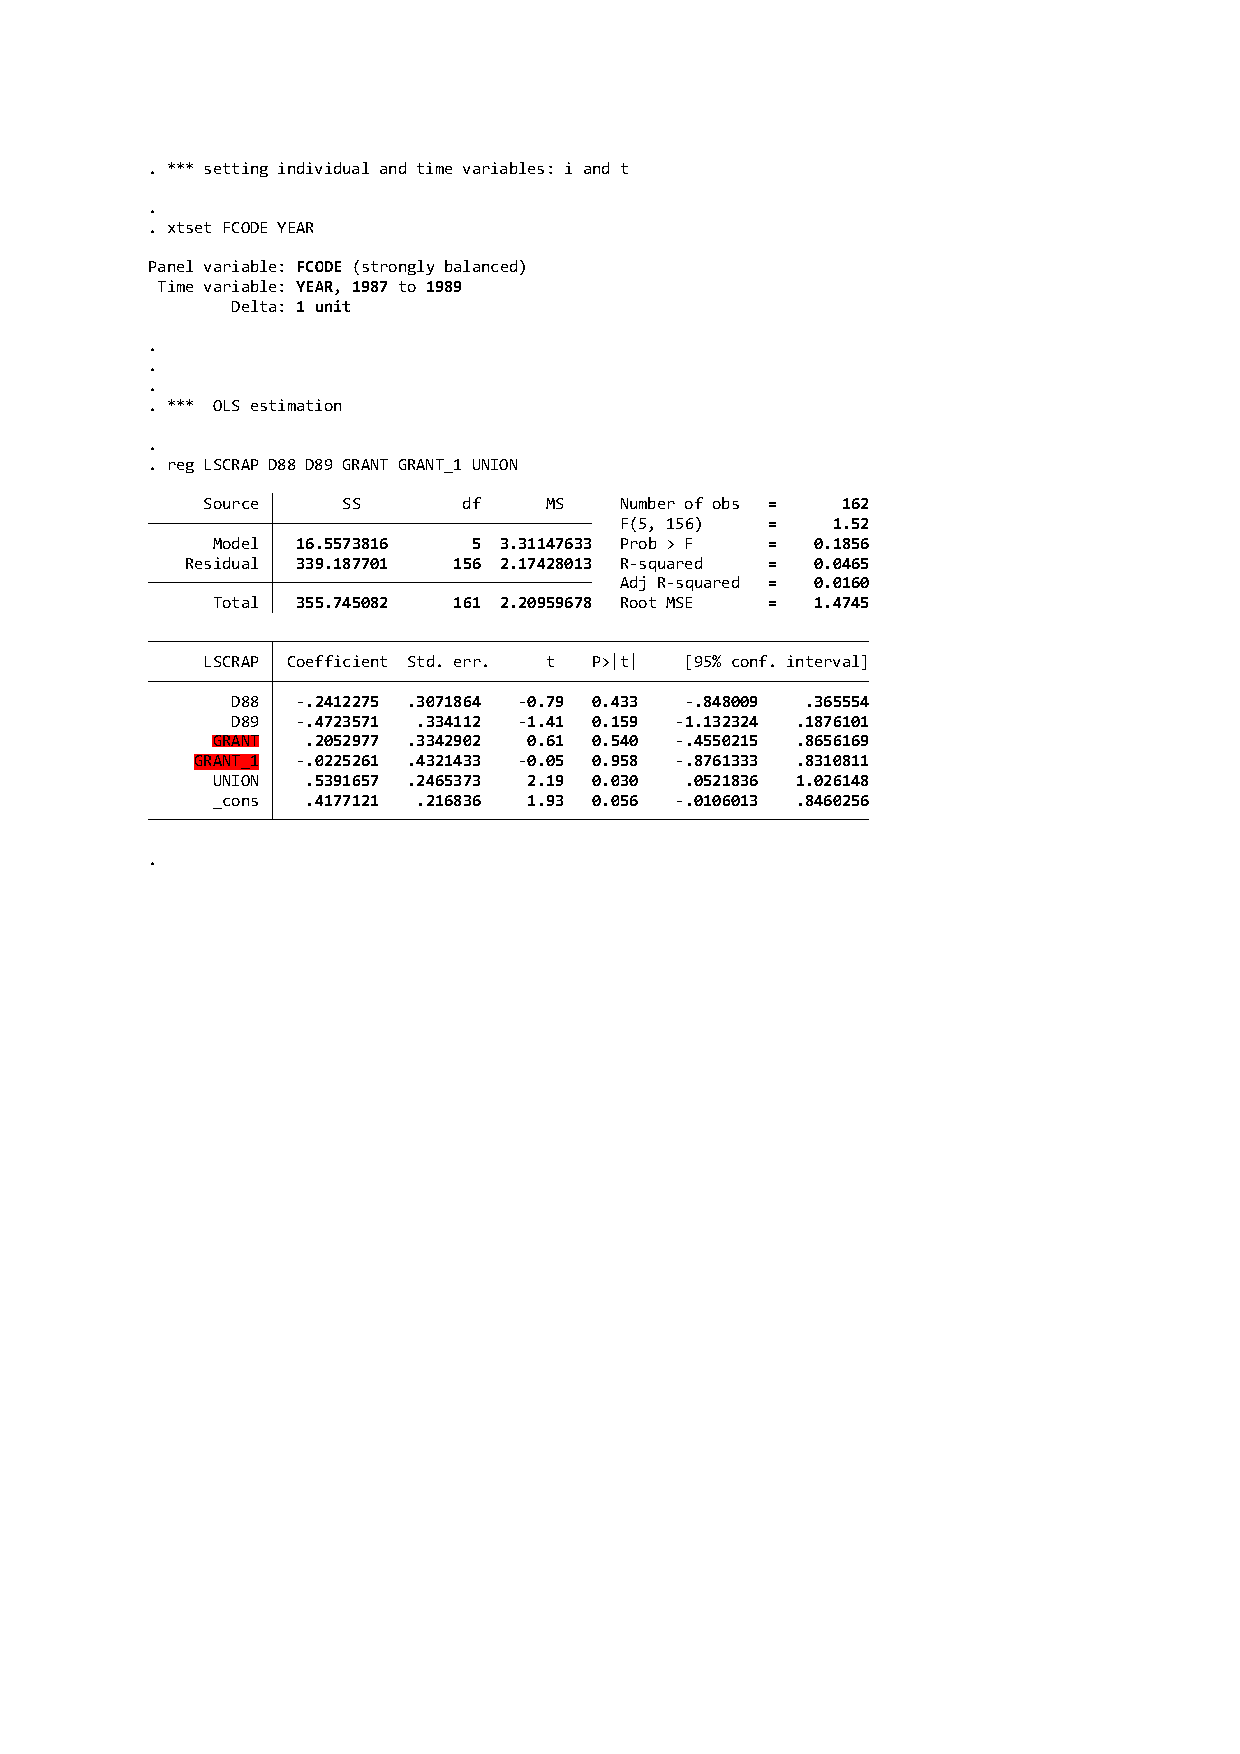
\includegraphics[width=0.9\textwidth]{hh1.pdf}
\end{figure}
\end{frame}

\begin{frame}{Fixed Effects vs. Random Effects}
\begin{enumerate}
\item[$\Rightarrow$] There are two modeling approaches based on the assumptions on~$\alpha_i$ and their interactions with~$\vx_{it}$
\item[$\Rightarrow$] {\bf Fixed effects model}:
\begin{itemize}
\item $\{ \alpha_i , i=1, \dots ,N \}$ are treated as fixed unknown parameters to be estimated
\item Consequently we have to deal with large number of parameters if $N$ is large
\item Allows $\E[x_{it} \alpha_i] \neq 0$ for some or all~$i$ and~$t$
\end{itemize}
\item[$\Rightarrow$] {\bf Random effects model}: 
\begin{itemize}
\item $\{ \alpha_i , i=1, \dots ,N \}$ are random
\item Assume, for each~$i$ and~$t$,
$$
\alpha_i \sim \text{i.i.d.}(0,\sigma_{\alpha}^2),\quad \E[x_{it}\alpha_i] = 0
$$
\item Instead of $N$ parameters there is only one ($\sigma_\alpha^2$)
\item Not always easy/possible to defend this assumption in practice 
\item Feasible generalized least squares leads to efficient estimates~$\hat\vbeta$
\end{itemize}
\end{enumerate}
\end{frame}

\begin{frame}{When Individual Effects Are Correlated With Regressors}
\begin{enumerate}
\item[$\Rightarrow$] Examples of how $\vx_{it}$ may be correlated with $\alpha_i$
\item[$\Rightarrow$] Individual earnings equation:
\begin{itemize}
\item $y_{it} = \log ( \text{wage}_{it})$
\item $\vx_{it}$ contains education level of individual~$i$
\item $\alpha_i$ includes unobserved ability, which is likely to affect~$\vx_{it}$
\end{itemize}
\item[$\Rightarrow$] Firm level investment equation:
\begin{itemize}
\item $y_{it} = \log ( \text{investment}_{it})$
\item $\vx_{it}$ contains cost of capital of firm~$i$
\item $\alpha_i$ includes unobserved managerial quality, which is likely to affect~$\vx_{it}$
\end{itemize}
\end{enumerate}
\end{frame}


%%%%%%%%%%%%%%%%%
\section{Fixed effects (FE) model}
%%%%%%%%%%%%%%%%%

\sectionframe{2}{Fixed Effects Model}

\begin{frame}{Fixed Effects: Setup}
\begin{enumerate}
\item[$\Rightarrow$] The FE model is a linear model with intercepts that vary across individuals/units ($i$)
$$
y_{it} = \alpha_i + \vx_{it}^{\prime}\vbeta + u_{it}, \quad u_{it}\sim\text{i.i.d.}(0,\sigma_u^2)
$$
\item[$\Rightarrow$] $\vx_{it}$ are independent of all $u_{it}$
\item[$\Rightarrow$] FE model treats unobserved heterogeneity $\alpha_i$ as parameters
\item[$\Rightarrow$] Direct estimators are less attractive when $N$ is large as it requires estimation of many parameters simultaneously (incidental parameter bias) 
\item[$\Rightarrow$] Alternatively, there are transformations of the model that eliminate $\alpha_i$ from the regression equation
\end{enumerate}
\end{frame}

\begin{frame}{The Within Transformation}
\begin{enumerate}
\item[$\Rightarrow$] The {\bf within transformation}:
\begin{itemize}
\item Take time-series averages of the FE regression model
$$
\frac{1}{T}\sum_{t=1}^T y_{it} = \alpha_i + \frac{1}{T}\sum_{t=1}^T \vx_{it}^{\prime}\vbeta + \frac{1}{T}\sum_{t=1}^T u_{it}
\quad \Rightarrow \quad
\bar{y}_i = \alpha_i + \bar\vx_i^{\prime} \vbeta + \bar{u}_i
$$
\item Calculate deviations from individual means, within model:
$$
y_{it}-\bar{y}_i = (\vx_{it}-\bar{\vx}_i)^{\prime} \vbeta + (u_{it}-\bar{u}_i )
$$
\vspace*{-\baselineskip}
\item Note: Cannot estimate coefficients on regressors that are constant over time, i.e.\ have $\vx_{it}=\bar{\vx}_i$
\end{itemize}
\item[$\Rightarrow$] The FE or ``within'' estimator is OLS applied to the transformed model, i.e.\
$$
\hat\vbeta_{\text{FE}} = \left(\sum_{i=1}^N \sum_{t=1}^T (\vx_{it}-\bar{\vx}_i ) (\vx_{it}-\bar{\vx}_i )^{\prime} \right)^{-1} \sum_{i=1}^N \sum_{t=1}^T (\vx_{it}-\bar{\vx}_i )(y_{it}-\bar{y}_i )
$$
\item[$\Rightarrow$] The $N$ intercepts are estimated as $\hat\alpha_i = \bar{y}_i - \bar\vx_i^{\prime} \hat\vbeta_{\text{FE}},i=1,\ldots ,N$
\end{enumerate}
\end{frame}

\begin{frame}{Least Squares Dummy Variables}
\begin{enumerate}
\item[$\Rightarrow$] Consider the least squares dummy variables (LSDV) estimator: 
\begin{itemize}
\item Jointly estimate the parameters $\alpha_1,\ldots, \alpha_N$ and $\vbeta$ by OLS
\item Define $\valpha = (\alpha_1,\ldots,\alpha_N )^{\prime}$
\item Let $\vd_i$ be a vector of size~$N$ with~1 as the $i$-th element and zeros elsewhere 
\item Write the model as 
$$
y_{it} = \vd_i^{\prime}\valpha + \vx_{it}^{\prime} \vbeta + u_{it}
$$
and run OLS to estimate $\valpha,\vbeta$
\item Numerically less appealing as it includes many regressors (handling very big matrices) 
\end{itemize}
\item[$\Rightarrow$] The ``within'' (or FE) method and the LSDV estimator are identical (by the FWL theorem)
\end{enumerate}
\end{frame}

\begin{frame}{Strict Exogeneity and FE Inference}
\begin{enumerate}
\item[$\Rightarrow$] The FE or within estimator requires the {\bf strict exogeneity condition}:
$$
\E[\vx_{it} u_{is}] = 0 \text{ for all~$s$ and~$t$}
$$
\vspace*{-\baselineskip}
\item[$\Rightarrow$] This assumption excludes, in particular, any dependence between $\vx_{it}$ and past values of $y_{it}$
\begin{itemize}
\item Hard to justify in practice
\item Example: Suppose we would like to explain labour supply of an individual using years of experience; then this would violate the strict exogeneity assumption because experience depends on the individual's labor history
\end{itemize}
\item[$\Rightarrow$] Covariance matrix of $\hat\vbeta_{\text{FE}}$:
\begin{align*}
\widehat\var[\hat\vbeta_{\text{FE}}] &= \hat\sigma_u^2 \left( \sum_{i=1}^N \sum_{t=1}^T (\vx_{it} - \bar\vx_i ) (\vx_{it} - \bar\vx_i )^{\prime} \right)^{-1} \\
\hat\sigma_u^2 &= \frac{1}{N(T-1)} \sum_{i=1}^N \sum_{t=1}^T \hat{u}_{it}^2
\quad \text{and} \quad
\hat{u}_{it} = y_{it} - \hat\alpha_i - \vx_{it}^{\prime} \hat\vbeta_{\text{FE}}
\end{align*}
\end{enumerate}
\end{frame}

\begin{frame}{Running Example: FE Within Estimator}
\framesubtitle{FE within estimator}
\vspace*{-1.6cm}
\begin{figure}
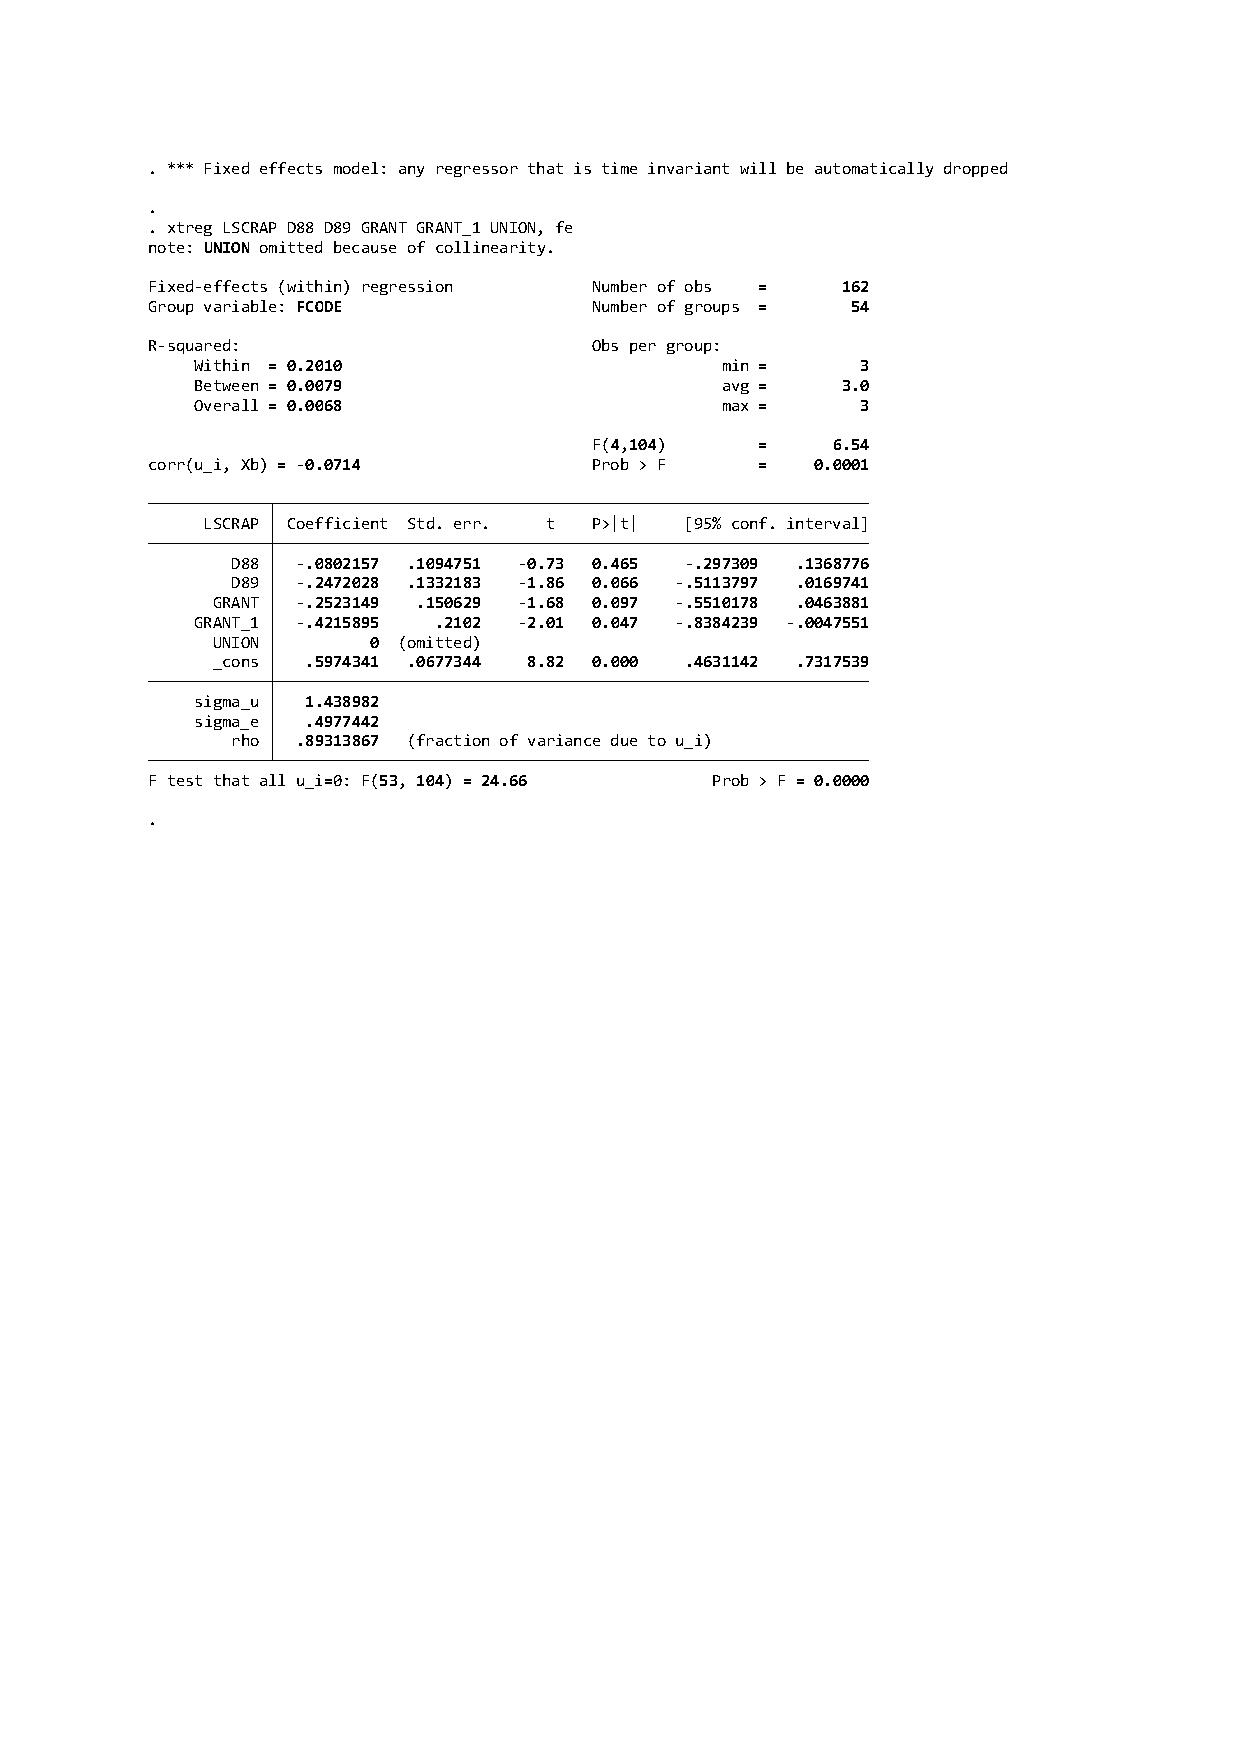
\includegraphics[width=0.9\textwidth]{hh3.pdf}
\end{figure}
\end{frame}

\begin{frame}{The Between Estimator}
\begin{enumerate}
\item[$\Rightarrow$] A related estimator is the ``between'' estimator obtained by OLS on the time averages, i.e.\ OLS on the regression
$$
\bar{y}_i = \beta_0 + \bar\vx_i^{\prime} \vbeta + \underbrace{\alpha_i + \bar{u}_i}_{\bar\varepsilon_i}
$$
\vspace*{-\baselineskip}
\item[$\Rightarrow$] The ``between'' estimator is then
$$
\hat\vbeta_{\text{B}} = \left(\sum_{i=1}^N (\bar\vx_i - \bar\vx ) (\bar\vx_i - \bar\vx )^{\prime} \right)^{-1} \sum_{i=1}^N (\bar\vx_i - \bar\vx )(\bar{y}_i - \bar{y} )
$$
\begin{itemize}
\item Compare with the ``within''/FE estimator
\end{itemize}
\item[$\Rightarrow$] Requires strict exogeneity, but also that $\alpha_i$ and $\vx_{it}$ are uncorrelated (strong assumptions)
\begin{itemize}
\item Last condition is not required by ``within''/FE estimator
\end{itemize}
\item[$\Rightarrow$] In fact, the ``between'' estimator is really only useful in the context of the RE model later
\end{enumerate}
\end{frame}

\begin{frame}{The First-Difference Estimator}
\begin{enumerate}
\item[$\Rightarrow$] The within transformation is not the only way to eliminate $\alpha_i$
\item[$\Rightarrow$] Recall the FE model:
$$
y_{it} = \alpha_i + \vx_{it}^{\prime} \vbeta + u_{it}, \quad u_{it}\sim\text{i.i.d.}(0,\sigma_u^2)
$$
\vspace*{-1.1\baselineskip}
\item[$\Rightarrow$] The first difference estimator for $\vbeta$:
\begin{itemize}
\item Take first differences,
$$
\hspace*{-1.25cm}
y_{it}-y_{i,t-1} = (\vx_{it}-\vx_{i,t-1})^{\prime}\vbeta+(u_{it}-u_{i,t-1})
\quad \Rightarrow  \quad
\Delta y_{it} = \Delta \vx_{it}^{\prime} \vbeta + \Delta u_{it}
$$
\vspace*{-1.1\baselineskip}
\item Estimate by OLS
\item Only $T-1$ observations in time dimension (lose one observation)
\item Standard errors of $\hat\vbeta_\text{FD}$ need to take into account that $\Delta u_{it}$ has serial correlation by construction
\item Note: Like FE/within estimator, cannot estimate coefficients on regressors that are constant over time, i.e.\ have $\Delta\vx_{it}=0$
\end{itemize}
\item[$\Rightarrow$] First difference estimator requires {\bf weak exogeneity condition}:
$$
\E[\Delta \vx_{it} \Delta  u_{it}] = 0 \text{ for all $t$}
$$
\vspace*{-1.1\baselineskip}
\begin{itemize}
\item Weaker than strict exogeneity required for within estimator
\end{itemize}
\end{enumerate}
\end{frame}

\begin{frame}{Running Example: First Differences}
\framesubtitle{FE first difference estimator}
\vspace*{-1.6cm}
\begin{figure}
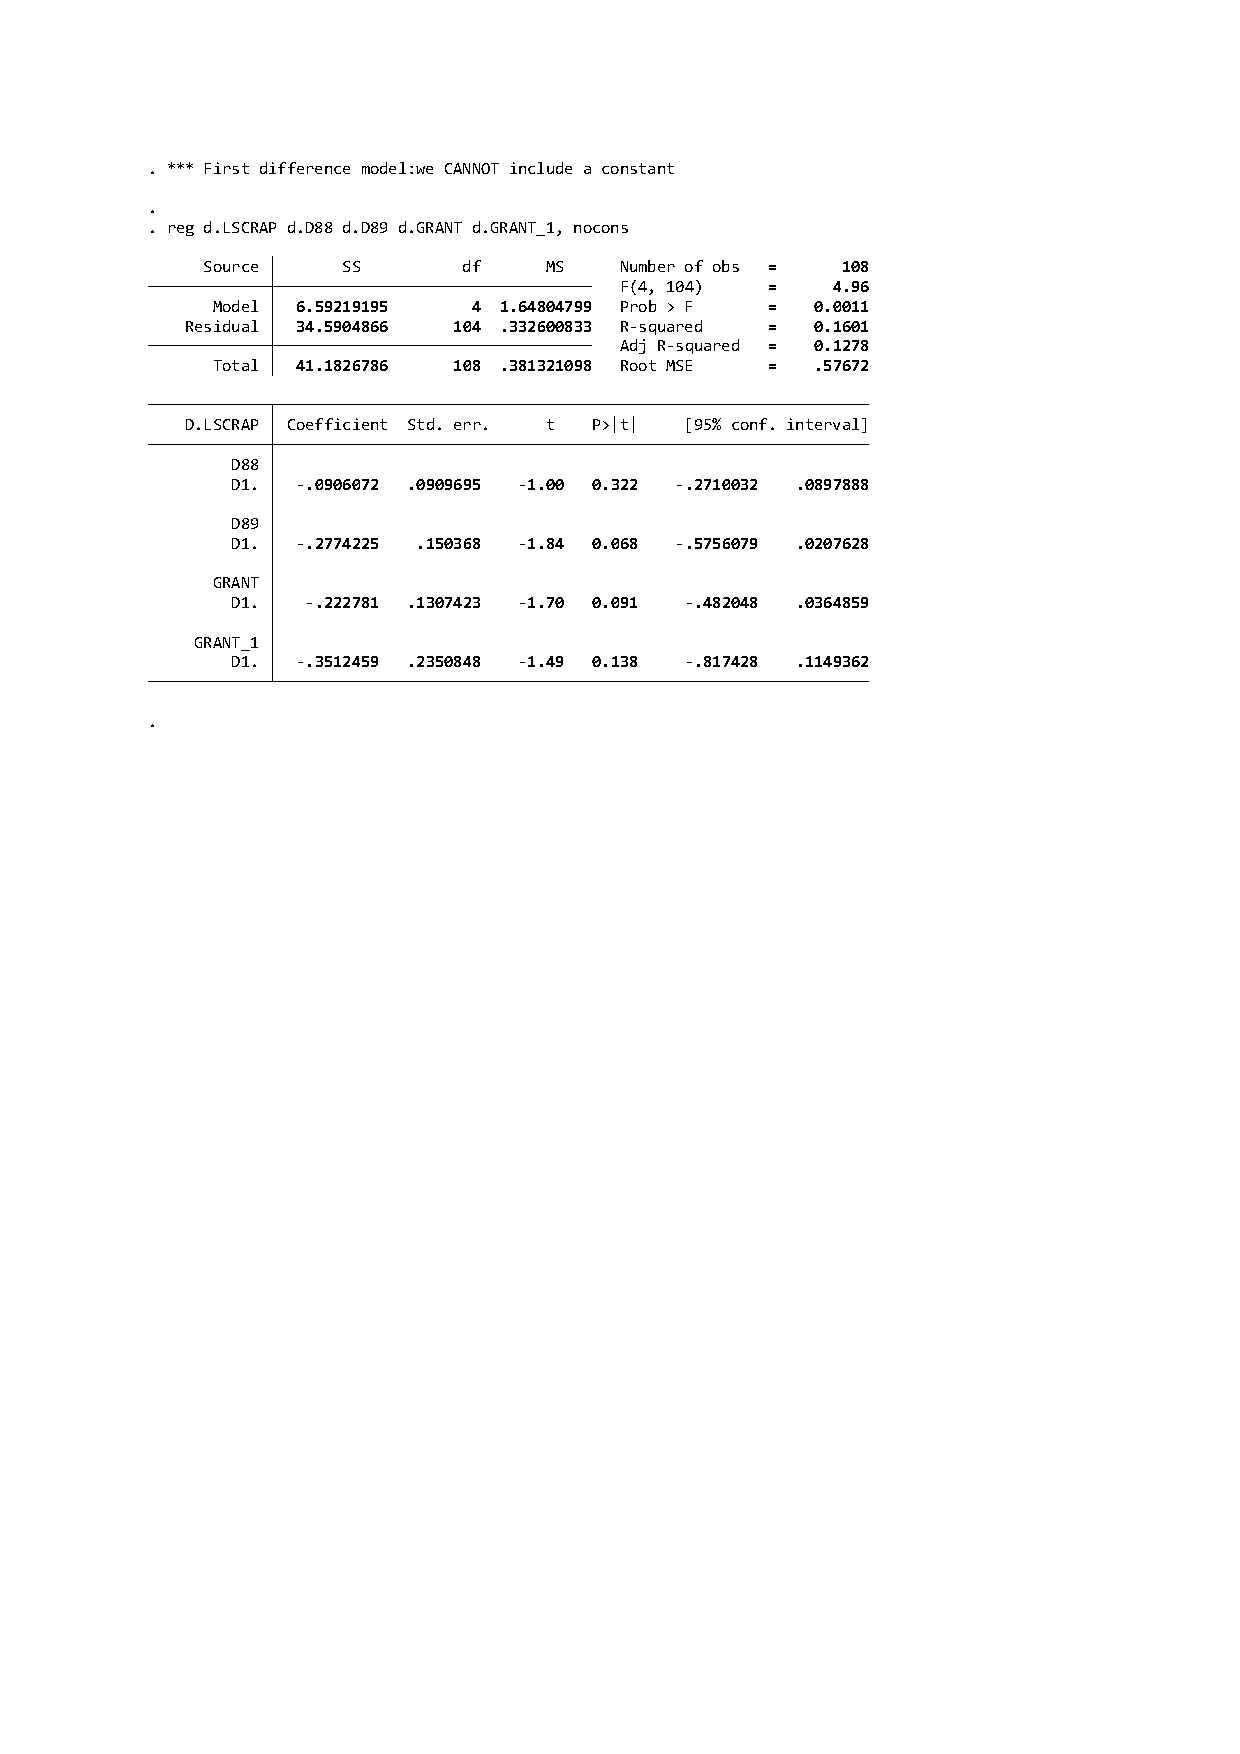
\includegraphics[width=\textwidth]{hh4.pdf}
\end{figure}
\end{frame}


%%%%%%%%%%%%%%%%%
\section{Random effects (RE) model}
%%%%%%%%%%%%%%%%%

\sectionframe{3}{Random Effects Model}

\begin{frame}{Random Effects: Setup}
\begin{enumerate}
\item[$\Rightarrow$] The RE model explicitly models $\alpha_i$ as a random variable (part of the error term)
\item[$\Rightarrow$] The RE model is thus
\begin{align*}
y_{it} &= \beta_0 + \vx_{it}^{\prime} \vbeta + \alpha_i + u_{it}\\
u_{it} &\sim\text{i.i.d.}(0,\sigma_u^2)\\
\alpha_i &\sim\text{i.i.d.}(0,\sigma_{\alpha}^2)
\end{align*}
\vspace*{-\baselineskip}
\begin{itemize}
\item $\alpha_i$ and $u_{it}$ are mutually independent
\item $\alpha_i$ and $u_{it}$ are independent from $\vx_{js}$ for each~$j$ and~$s$ (even stronger than strict exogeneity)
\end{itemize}
\item[$\Rightarrow$] (Pooled) OLS estimator of $\beta_0, \vbeta$ is consistent but:
\begin{itemize}
\item The usual standard errors are wrong (serial correlation in errors induced by $\alpha_i$) 
\item OLS is not efficient as it does not take advantage of the particular form of the error covariance matrix 
\end{itemize}
\item[$\Rightarrow$] For the price of the exogeneity condition we can obtain more efficient estimator
\end{enumerate}
\end{frame}

\begin{frame}{Random Effects: GLS Intuition}
\begin{enumerate}
\item[$\Rightarrow$] Hence we develop the {\bf Generalized Least Squares (GLS)} estimator that explores the particular error structure
\item[$\Rightarrow$] Intuition behind GLS: apply OLS to a transformed data such that covariance matrix of the transformed error is an identity matrix
\item[$\Rightarrow$] Define $\vu_i = (u_{i1},\ldots,u_{iT})^{\prime}$, $\viota_T = (1,1,\ldots,1)^{\prime}$, and the $T\times T$ identity matrix~$\mI_T$
\item[$\Rightarrow$] The composite error term is then $\vvarepsilon_i = \alpha_i \viota_T +\vu_i$
\item[$\Rightarrow$] Write model as (ignoring constant term or including it in~$\vx_i$)
$$
\underbrace{\vy_i}_{T\times 1} = \underbrace{\mX_i^{\prime}}_{T\times K}\underbrace{\vbeta}_{K\times 1}+\underbrace{\vvarepsilon_i}_{T\times 1}
\quad \text{with} \quad \E[\vvarepsilon_i] = \vzeros ,
\quad \var[\vvarepsilon_i] = \underbrace{\mOmega}_{T\times T}
$$
where $\vy_i = (y_{i1},\ldots,y_{iT})^{\prime}$ and $\mX_i = (\vx_{i1},\ldots,\vx_{iT})$
\item[$\Rightarrow$] If we knew the matrix $\mOmega$ then OLS on the transformed model
$$
\mOmega^{-1/2}\vy_i = \mOmega^{-1/2}\mX_i^{\prime}\vbeta + \mOmega^{-1/2}\vvarepsilon_i 
$$
gives the GLS estimator
\end{enumerate}
\end{frame}

\begin{frame}{Random Effects: GLS Estimator}
\begin{enumerate}
\item[$\Rightarrow$] If we knew $\mOmega$ then 
$$
\hat\vbeta_{\text{GLS}} = \left(\sum_{i=1}^N \mX_i \mOmega^{-1} \mX_i^{\prime}\right)^{-1} \sum_{i=1}^N \mX_i \mOmega^{-1} \vy_i 
$$
\item[$\Rightarrow$] Under normality (and conditional on $\mX$),
$$
\hat\vbeta_{\text{GLS}} \sim \rN \left( \vbeta , \left(\sum_{i=1}^N \mX_i \mOmega^{-1} \mX_i^{\prime} \right)^{-1}\right)
$$
\item[$\Rightarrow$] Also holds without normality, but then only asymptotically 
\item[$\Rightarrow$] Follows from standard linear manipulations and by noting that $\E[\sum_{i=1}^N \mX_i \mOmega^{-1} \vvarepsilon_i \vvarepsilon_i^{\prime} \mOmega^{-1} \mX_i^{\prime} |\mX] =\sum_{i=1}^N \mX_i \mOmega^{-1} \mX_i^{\prime}$
\item[$\Rightarrow$] So we need to find $\mOmega$....
\end{enumerate}
\end{frame}

\begin{frame}{Random Effects: Error Covariance Matrix}
\begin{align*}
\mOmega = \var[\vvarepsilon_i] 
&= \var[\alpha_i \viota_T + \vu_i] \\
&= \sigma_{\alpha}^2\viota_T\viota_T^{\prime} + \sigma_u^2\mI_T \\
&= \left(
\begin{array}{cccccc}
\sigma^2_\alpha+\sigma_u^2&\sigma_\alpha^2&\dots&\sigma_\alpha^2\\
\sigma_\alpha^2&\sigma^2_\alpha+\sigma_u^2&\dots&\sigma_\alpha^2\\
\vdots&\vdots&\ddots&\vdots\\
\sigma_\alpha^2&\sigma_\alpha^2&\dots&\sigma^2_\alpha+\sigma_u^2
\end{array}
\right)
\end{align*}
\begin{itemize}
\item[$\Rightarrow$] This matrix has $\sigma^2_\alpha+\sigma_u^2$ on the diagonal and $\sigma_\alpha^2$ elsewhere
\item[$\Rightarrow$] Need estimates of $\sigma^2_\alpha$ and $\sigma_u^2$ to obtain feasible GLS estimator
\end{itemize}
\end{frame}

\begin{frame}{Random Effects: Quasi-Demeaning}
\begin{enumerate}
\item[$\Rightarrow$] With a ton of algebra, it is possible to show that 
\begin{align*}
\hat\vbeta_{\text{GLS}} ={}& \left( \sum_{i=1}^N \sum_{t=1}^T (\vx_{it} -\bar\vx_i )(\vx_{it} -\bar\vx_i )^\prime + \psi T \sum_{i=1}^N (\bar\vx_i - \bar\vx)(\bar\vx_i - \bar\vx)^\prime \right)^{-1} \\
&\times \left( \sum_{i=1}^N \sum_{t=1}^T (\vx_{it} -\bar\vx_i )(y_{it} -\bar{y}_i )^\prime + \psi T \sum_{i=1}^N (\bar\vx_i - \bar\vx)(\bar{y}_i - \bar{y})^\prime \right) ,
\end{align*}
where
$$
\psi = \frac{\sigma_u^2}{\sigma_u^2 + T \sigma_\alpha^2}
$$
\item[$\Rightarrow$] This is just an alternative derivation of the same estimator
\item[$\Rightarrow$] Possible computational advantage since we don't need to invert a big $T \times T$ matrix
\item[$\Rightarrow$] Still need estimates of $\sigma^2_\alpha$ and $\sigma_u^2$ to obtain feasible GLS estimator
\end{enumerate}
\end{frame}

\begin{frame}{RE - feasible GLS estimator}
\begin{enumerate}
\item[$\Rightarrow$] Using the FE (within) estimator we can estimate $\sigma_u^2$:
\begin{align*}
\hat{u}_{it} &= y_{it} - \hat\alpha_i - \vx_{it}^{\prime}\hat\vbeta_{\text{FE}} \\
\hat\sigma_u^2 &= \frac{1}{N(T-1)}\sum_{i=1}^N \sum_{t=1}^T \hat{u}_{it}^2
\end{align*}
\item[$\Rightarrow$] Using the ``between'' estimator we can then estimate $\sigma_\alpha^2$:
\begin{itemize}
\item Recall the between model: $\bar{y}_i = \beta_0 + \bar\vx_i^{\prime} \vbeta +\bar\varepsilon_i$
\item The variance of $\bar\varepsilon_i$ is $\var[\bar\varepsilon_i] = \var[\alpha_i + \bar{u}_i] = \sigma_\alpha^2+T^{-1}\sigma_u^2$
\item Then
$$
\frac{1}{N}\sum_{i=1}^N (\bar{y}_i - \hat\beta_{0,\text{B}} - \bar\vx_i^{\prime} \hat\vbeta_\text{B} )^2 
= \hat\sigma_\alpha^2 + \frac{1}{T} \hat\sigma_u^2
$$
\item Solve for $\hat\sigma_\alpha^2$
\end{itemize}
\item[$\Rightarrow$] Using these estimates yields the feasible GLS estimator - aka the {\bf random effects (RE) estimator}, $\hat\vbeta_{\text{RE}}$
\end{enumerate}
\end{frame}

\begin{frame}{Running Example: Random Effects}
\vspace*{-1.6cm}
\begin{figure}
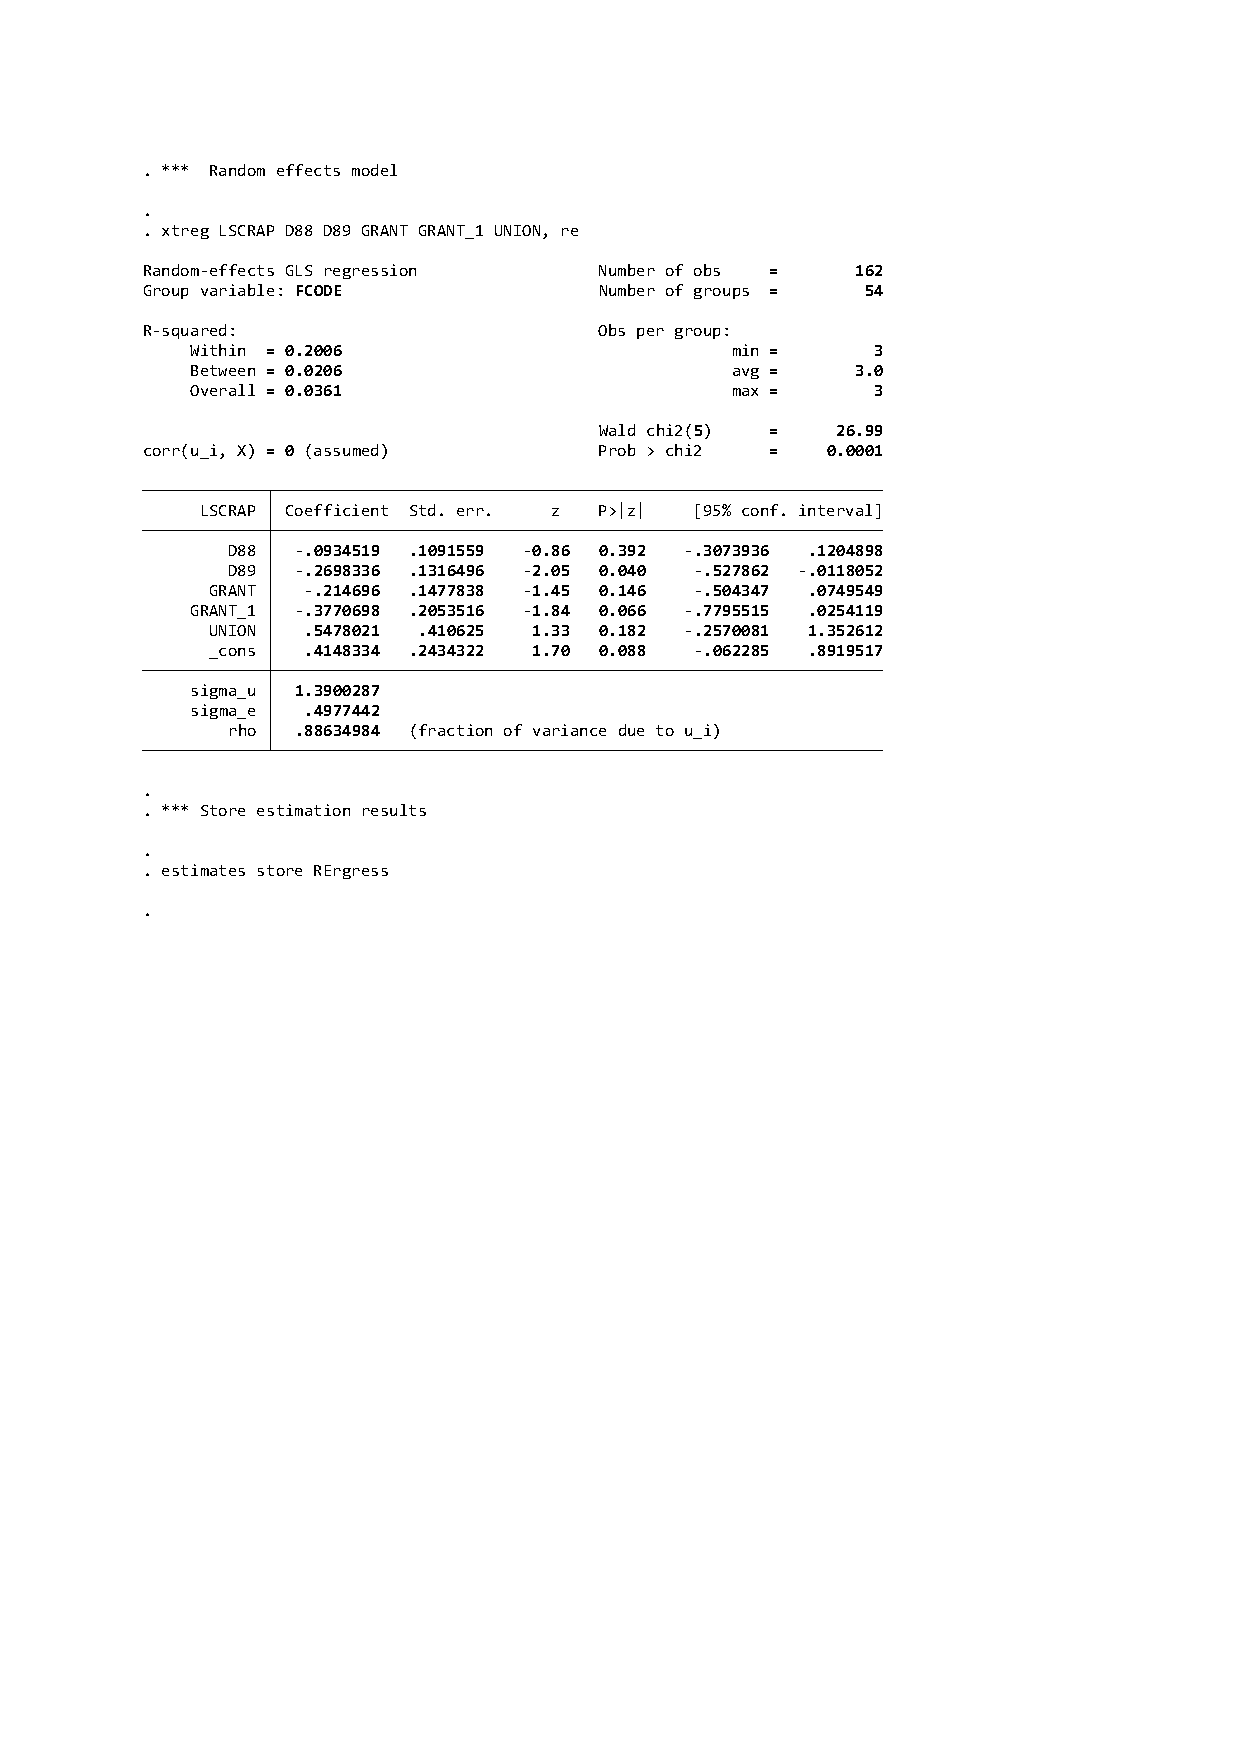
\includegraphics[width=\textwidth]{hh5.pdf}
\end{figure}
\end{frame}


%%%%%%%%%%%%%%%%%
\section{Cluster-robust inference}
%%%%%%%%%%%%%%%%%

\sectionframe{4}{Cluster-Robust Inference}

\begin{frame}{Cluster-Robust Standard Errors}
\begin{enumerate}
\item[$\Rightarrow$] Textbook section 10.2.7 discusses cluster-robust inference
\item[$\Rightarrow$] Generalization of White's heteroskedasticity-robust standard errors% (``robust'' in Stata)
\item[$\Rightarrow$] Non-panel case: suppose data can be divided into $G$ clusters
$$
\underbrace{\vy_g}_{N_g \times 1} = \underbrace{\mX_g^\prime}_{N_g \times K} \vbeta + \underbrace{\vu_g}_{N_g \times 1} , \quad g=1, \ldots , G
$$
\vspace*{-0.6\baselineskip}
\begin{itemize}
\item The clusters are independent of each other
\item We make no assumptions about dependence within clusters
\end{itemize}
\item[$\Rightarrow$] The variance of OLS estimator $\hat\vbeta = \vbeta_0 + (\mX^\prime \mX )^{-1} \sum_{g=1}^G \mX_g \vu_g$ is $(\mX^\prime \mX )^{-1} \sum_{g=1}^G \mX_g \mOmega_g \mX_g^\prime  (\mX^\prime \mX )^{-1}$, where $\mOmega_g = \var[\vu_g]$
\item[$\Rightarrow$] The cluster-robust variance estimator (CRVE) is
$$
\scalebox{0.9}{$\widehat\var[\hat\vbeta] = (\mX^\prime \mX )^{-1} \displaystyle\sum_{g=1}^G \mX_g \hat\vu_g \hat\vu_g^\prime \mX_g^\prime  (\mX^\prime \mX )^{-1}$}
$$
\vspace*{-0.6\baselineskip}
\item[$\Rightarrow$] MacKinnon, Nielsen, Webb (2023): ``Cluster-robust inference: A guide to empirical practice'', \emph{Journal of Econometrics}
\end{enumerate}
\end{frame}


%%%%%%%%%%%%%%%%%
\section{FE vs.\ RE models - Hausman test}
%%%%%%%%%%%%%%%%%

\sectionframe{5}{FE vs. RE Models: Hausman Test}

\begin{frame}{FE vs.\ RE: Hausman Test Intuition}
\begin{enumerate}
\item[$\Rightarrow$] It is hard to choose between the FE and RE estimators
\item[$\Rightarrow$] One criterion can be built upon whether $\alpha_i$ and $\vx_{it}$ are uncorrelated
\item[$\Rightarrow$] Hausman test is built on this logic 
\item[$\Rightarrow$] General idea of a Hausman test:
\begin{itemize}
\item Suppose you have two estimators, $\hat\theta_A$ and $\hat\theta_B$
\item Under one hypothesis, both $\hat\theta_A$ and $\hat\theta_B$ are consistent, but $\hat\theta_A$ is more efficient than $\hat\theta_B$
\item Under the other hypothesis, $\hat\theta_A$ is inconsistent and $\hat\theta_B$ is consistent
\item Intuition: $\hat\theta_A$ is efficient under ideal circumstances, but not robust, and $\hat\theta_B$ is robust, but not efficient
\end{itemize}
\item[$\Rightarrow$] In the present setup, suppose $\E[u_{it} \vx_{is}] =0$ for all $t$ and $s$, so that:
\begin{itemize}
\item If $\alpha_i$ and $\vx_{it}$ are uncorrelated then both $\hat\vbeta_{\text{FE}}$ and $\hat\vbeta_{\text{RE}}$ are consistent, but $\hat\vbeta_{\text{RE}}$ is more efficient
\item If $\alpha_i$ and $\vx_{it}$ are correlated then $\hat\vbeta_{\text{RE}}$ is inconsistent while $\hat\vbeta_{\text{FE}}$ is still consistent
\end{itemize}
\end{enumerate}
\end{frame}

\begin{frame}{FE vs.\ RE: Hausman Test Statistic}
\begin{enumerate}
\item[$\Rightarrow$] Hausman test formally...
\item[$\Rightarrow$] Under the null of the test, $\alpha_i$ and $\vx_{it}$ are uncorrelated
\item[$\Rightarrow$] This implies that both $\hat\vbeta_{\text{RE}}$ and $\hat\vbeta_{\text{FE}}$ are consistent, hence the distance $\hat\vbeta_{\text{FE}}-\hat\vbeta_{\text{RE}}$ must not be significantly different from zero
\item[$\Rightarrow$] If $\hat\vbeta_{\text{FE}}-\hat\vbeta_{\text{RE}}$ is statistically significantly different from zero, then $\alpha_i$ and $\vx_{it}$ are correlated
\item[$\Rightarrow$] Test statistic is
$$
\xi_\text{H} = (\hat\vbeta_{\text{FE}}-\hat\vbeta_{\text{RE}})^{\prime}\left(\widehat\var[\hat\vbeta_{\text{FE}}]-\widehat\var[\hat\vbeta_{\text{RE}}]\right)^{-1}(\hat\vbeta_{\text{FE}}-\hat\vbeta_{\text{RE}})
$$
\item[$\Rightarrow$] Under the null, $\xi_\text{H}\sim\chi^2(K)$ asymptotically, where $\chi^2 (K)$ is a chi-squared distribution with $K$ degrees of freedom
\item[$\Rightarrow$] Note that we used the curious result that $\var[\hat\vbeta_{\text{FE}}-\hat\vbeta_{\text{RE}}] = \var[\hat\vbeta_{\text{FE}}]-\var[\hat\vbeta_{\text{RE}}]$ under the null
\item[$\Rightarrow$] If test rejects, then use $\hat\vbeta_{\text{FE}}$, otherwise use $\hat\vbeta_{\text{RE}}$
\end{enumerate}
\end{frame}

\begin{frame}{Running Example: Hausman Test}
\vspace*{-1.6cm}
\begin{figure}
\hspace*{-1.5cm}
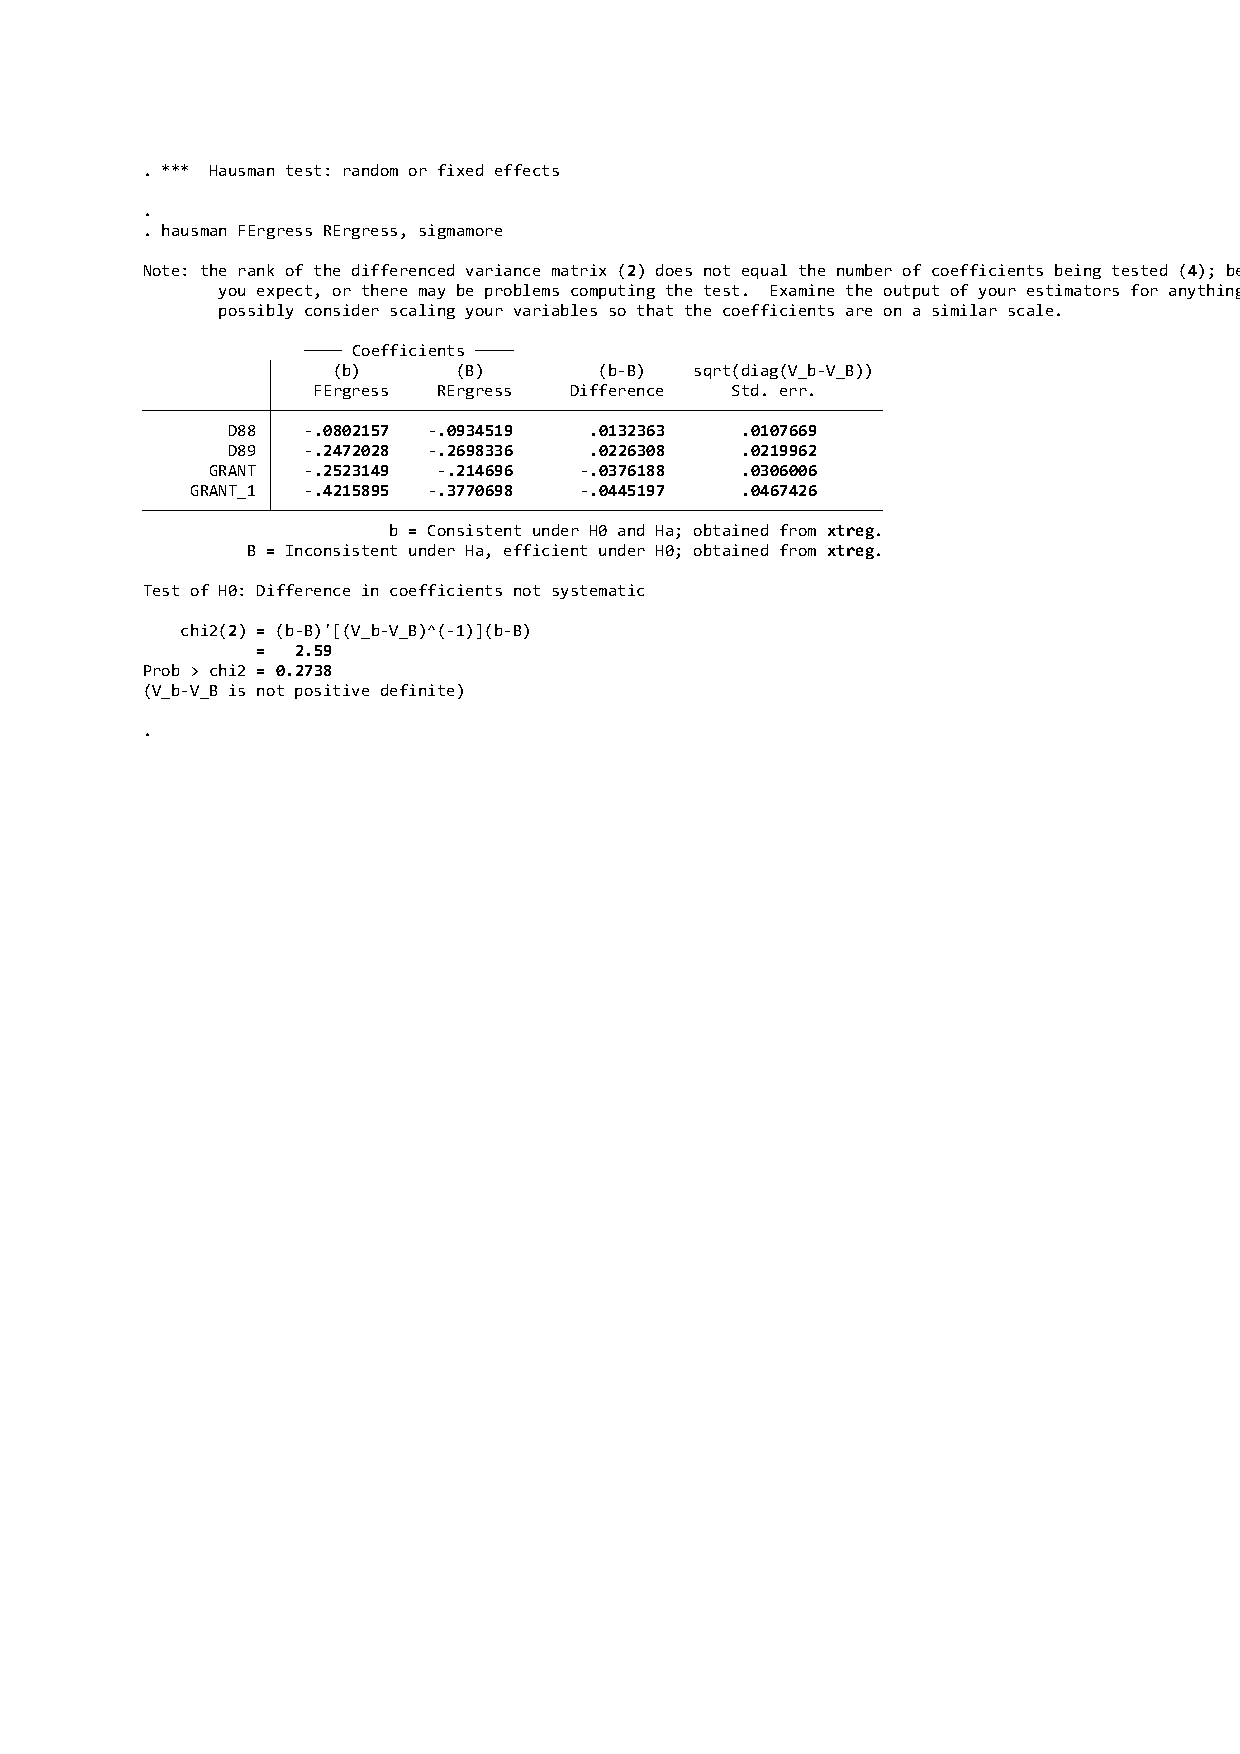
\includegraphics[width=\textwidth]{hh6.pdf}
\end{figure}
\end{frame}

%%%%%%%%%%%%%%%%%
\section{Grunfeld example}
%%%%%%%%%%%%%%%%%

\sectionframe{6}{Grunfeld Example}

\begin{frame}{Grunfeld (1958) investment equation}
\begin{enumerate}
\item[$\Rightarrow$] Grunfeld, Y.\ (1958), \emph{The Determinants of Corporate Investment}, Ph.D.\ thesis, Department of Economics, University of Chicago
\item[$\Rightarrow$] Old, but famous example in all the textbooks; e.g.\\
Baltagi (2021), \emph{Econometric Analysis of Panel Data}, 4th edition
\item[$\Rightarrow$] Consider the following investment equation
$$
I_{it} = \alpha_i + \beta_1 F_{it} + \beta_2 C_{it} + u_{it}
$$
\begin{itemize}
\item $I_{it}$ denotes real gross investment for firm~$i$ in year~$t$
\item $F_{it}$ is the real value of a firm 
\item $C_{it}$ is the real value of the capital stock
\item $N=10$ large US manufacturing firms are observed over $T=20$ years, 1935--1954
\end{itemize}
\end{enumerate}
\end{frame}

\begin{frame}{Grunfeld - pooled panel OLS}
\vspace*{-1.75cm}
\begin{figure}
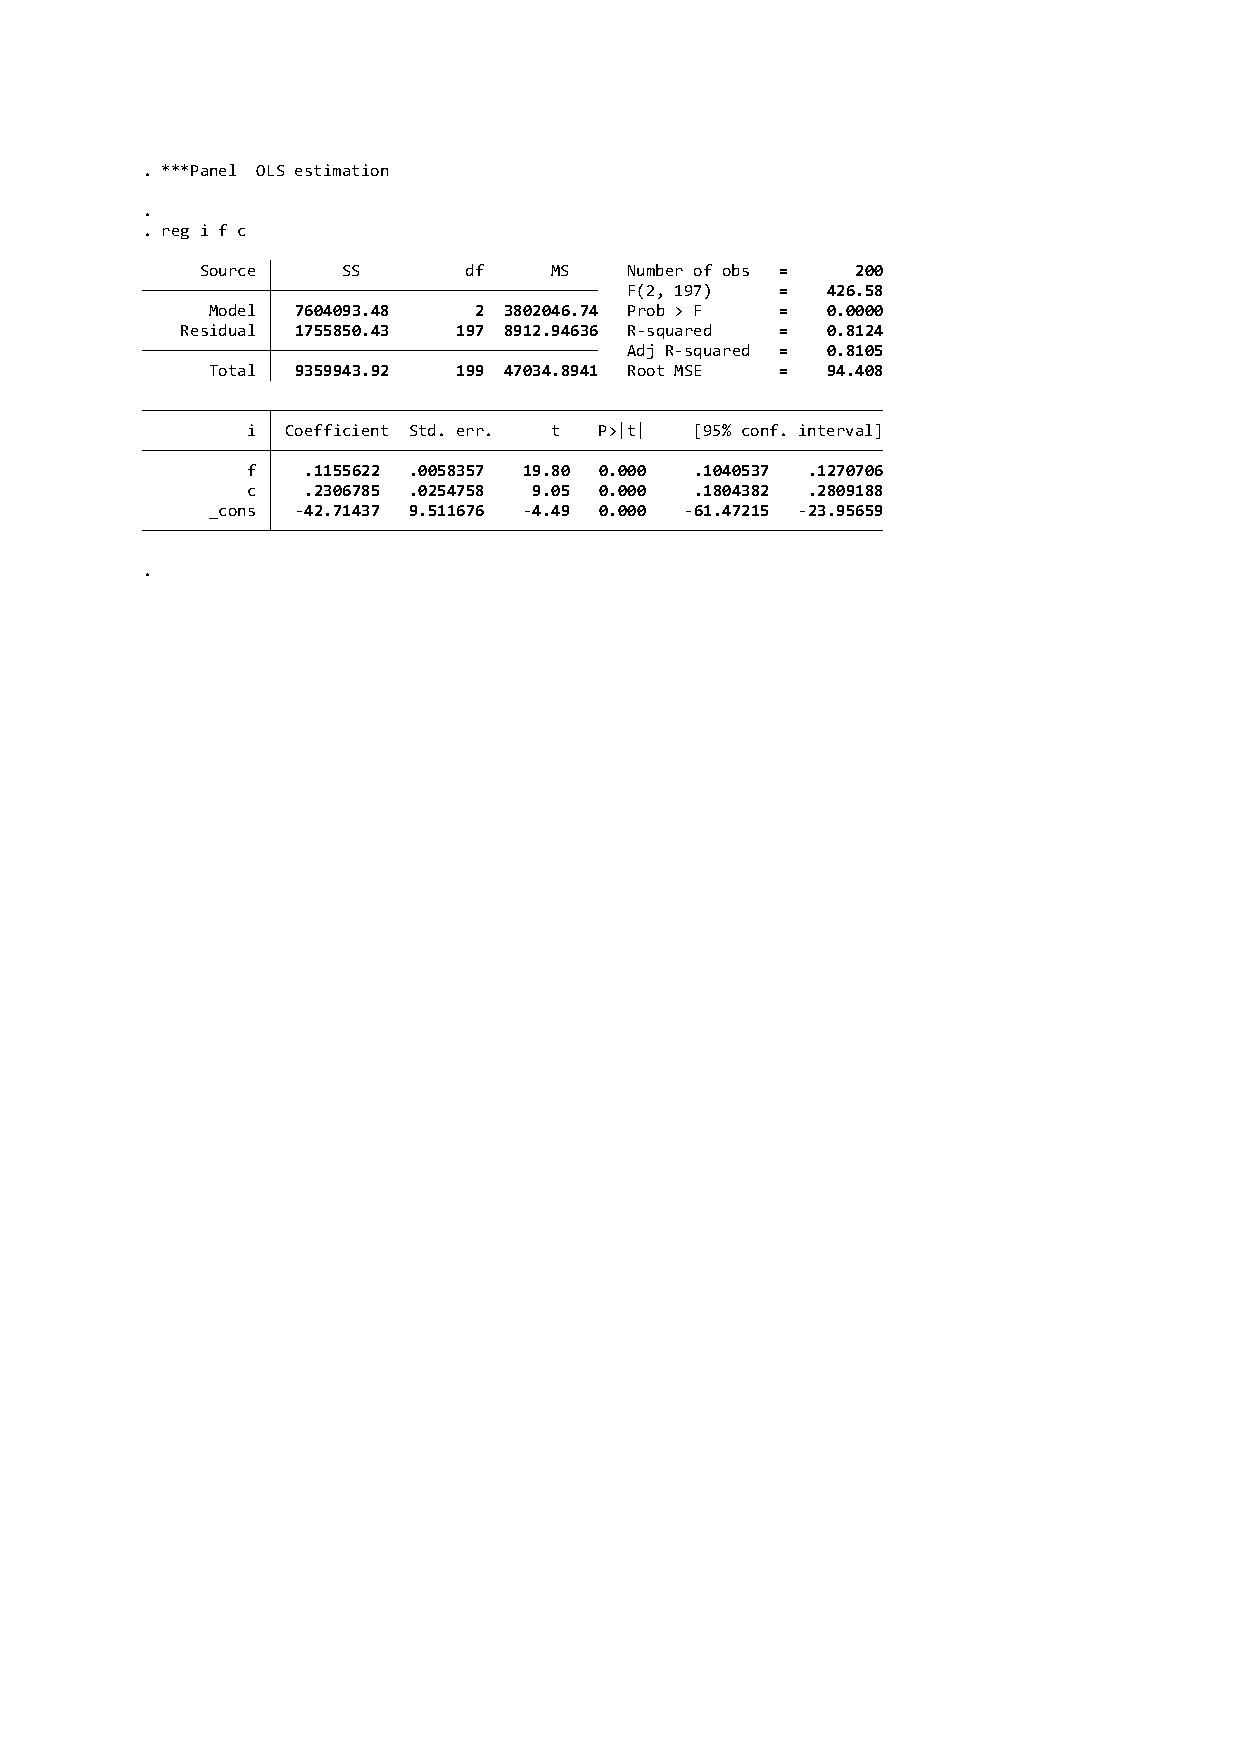
\includegraphics[width=\textwidth]{hh7.pdf}
\end{figure}
\end{frame}

\begin{frame}{Grunfeld - panel FE estimator}
\vspace*{-1.75cm}
\begin{figure}
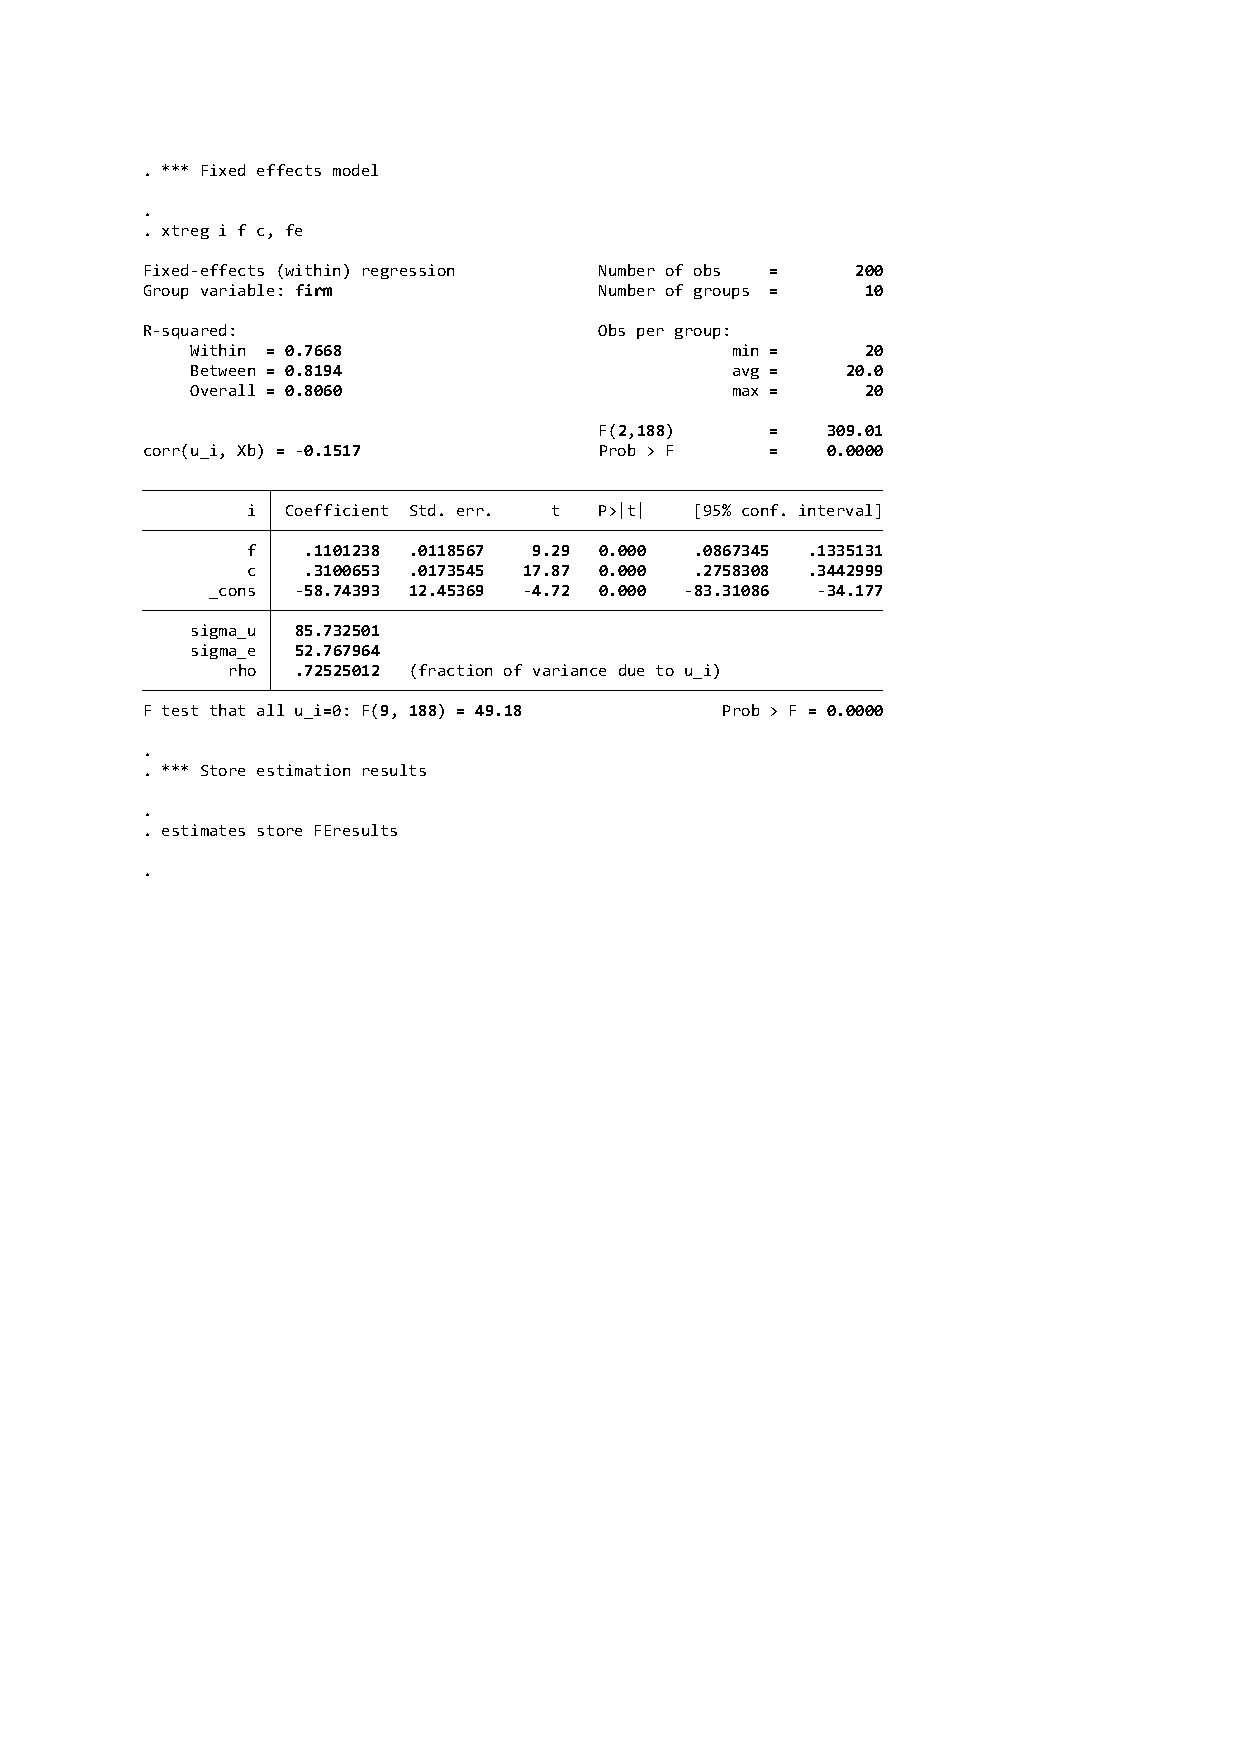
\includegraphics[width=0.9\textwidth]{hh8.pdf}
\end{figure}
\end{frame}

\begin{frame}{Grunfeld - panel RE estimator}
\vspace*{-1.75cm}
\begin{figure}
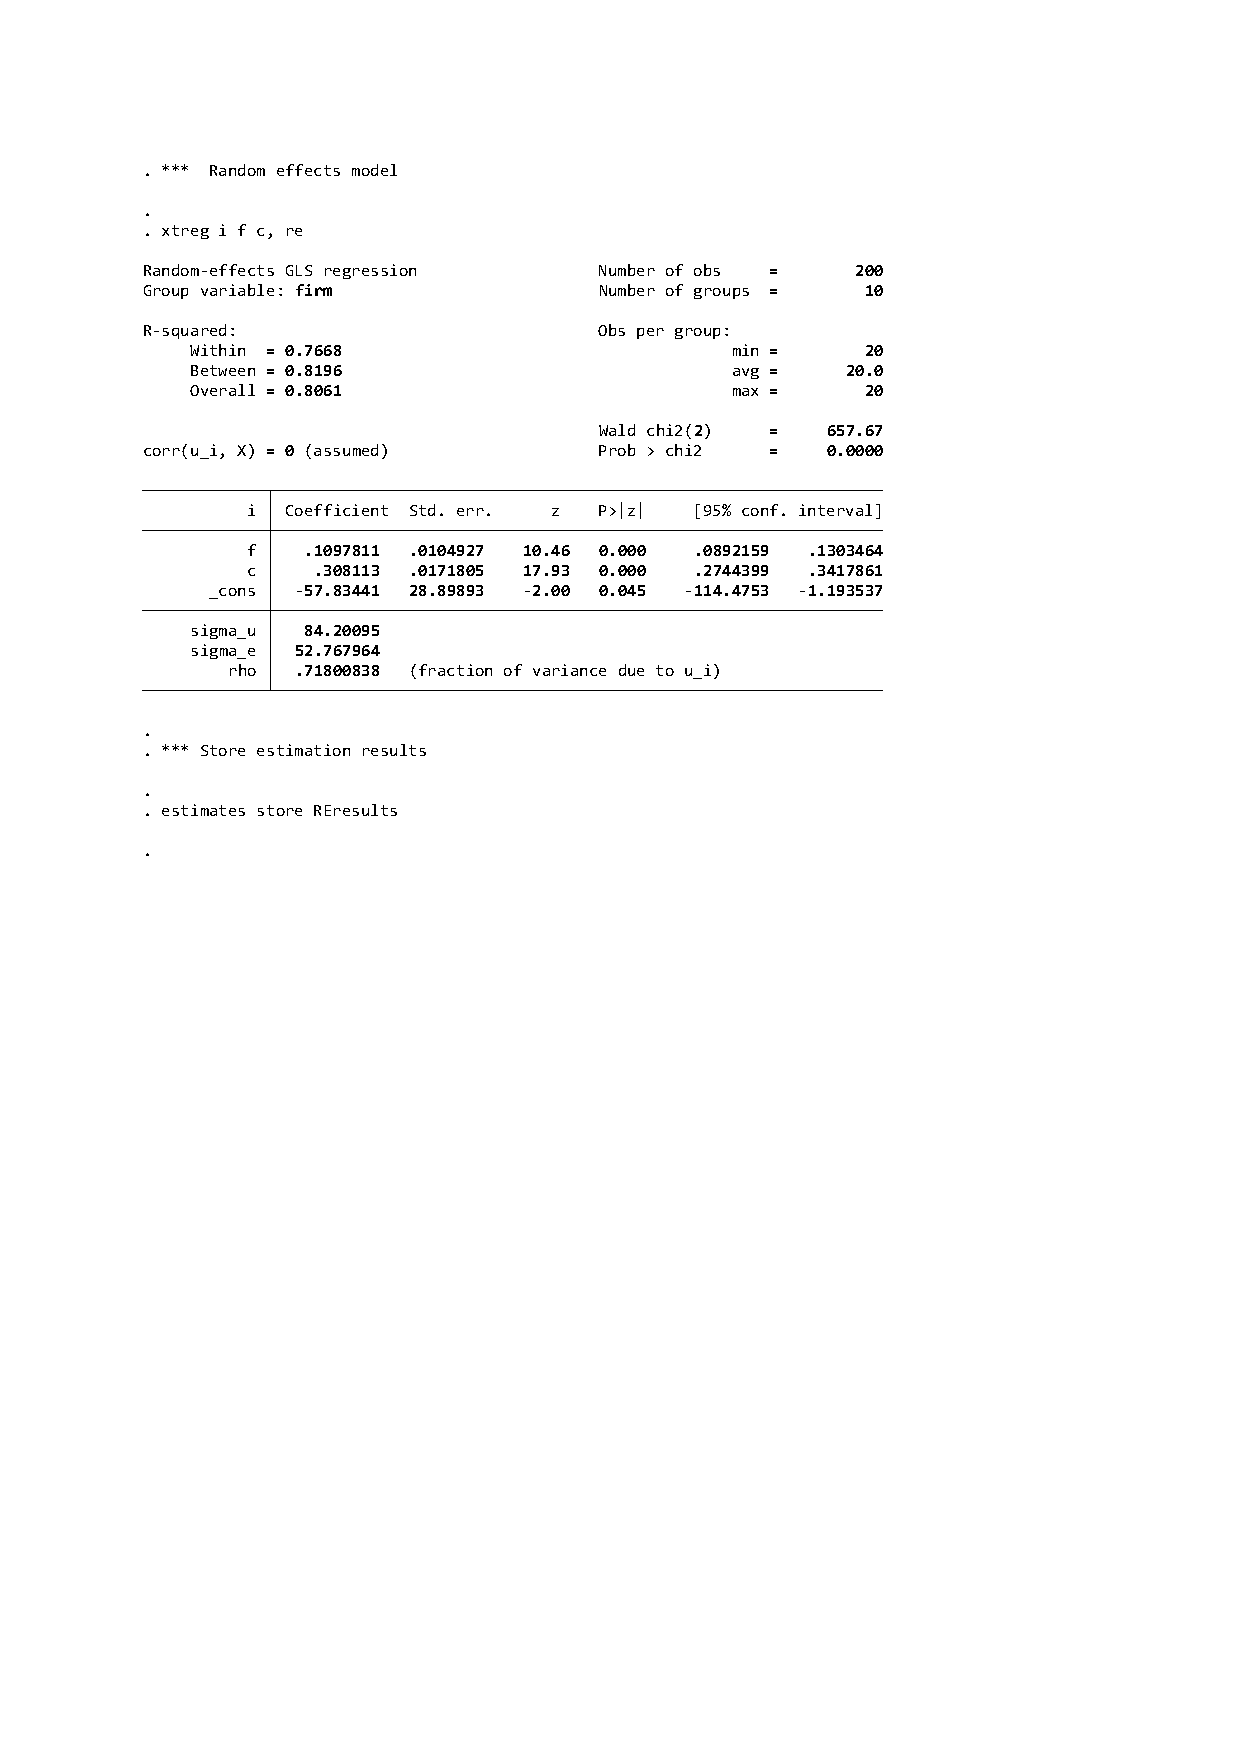
\includegraphics[width=0.9\textwidth]{hh9.pdf}
\end{figure}
\end{frame}

\begin{frame}{Grunfeld - Hausman test}
\vspace*{-1.75cm}
\begin{figure}
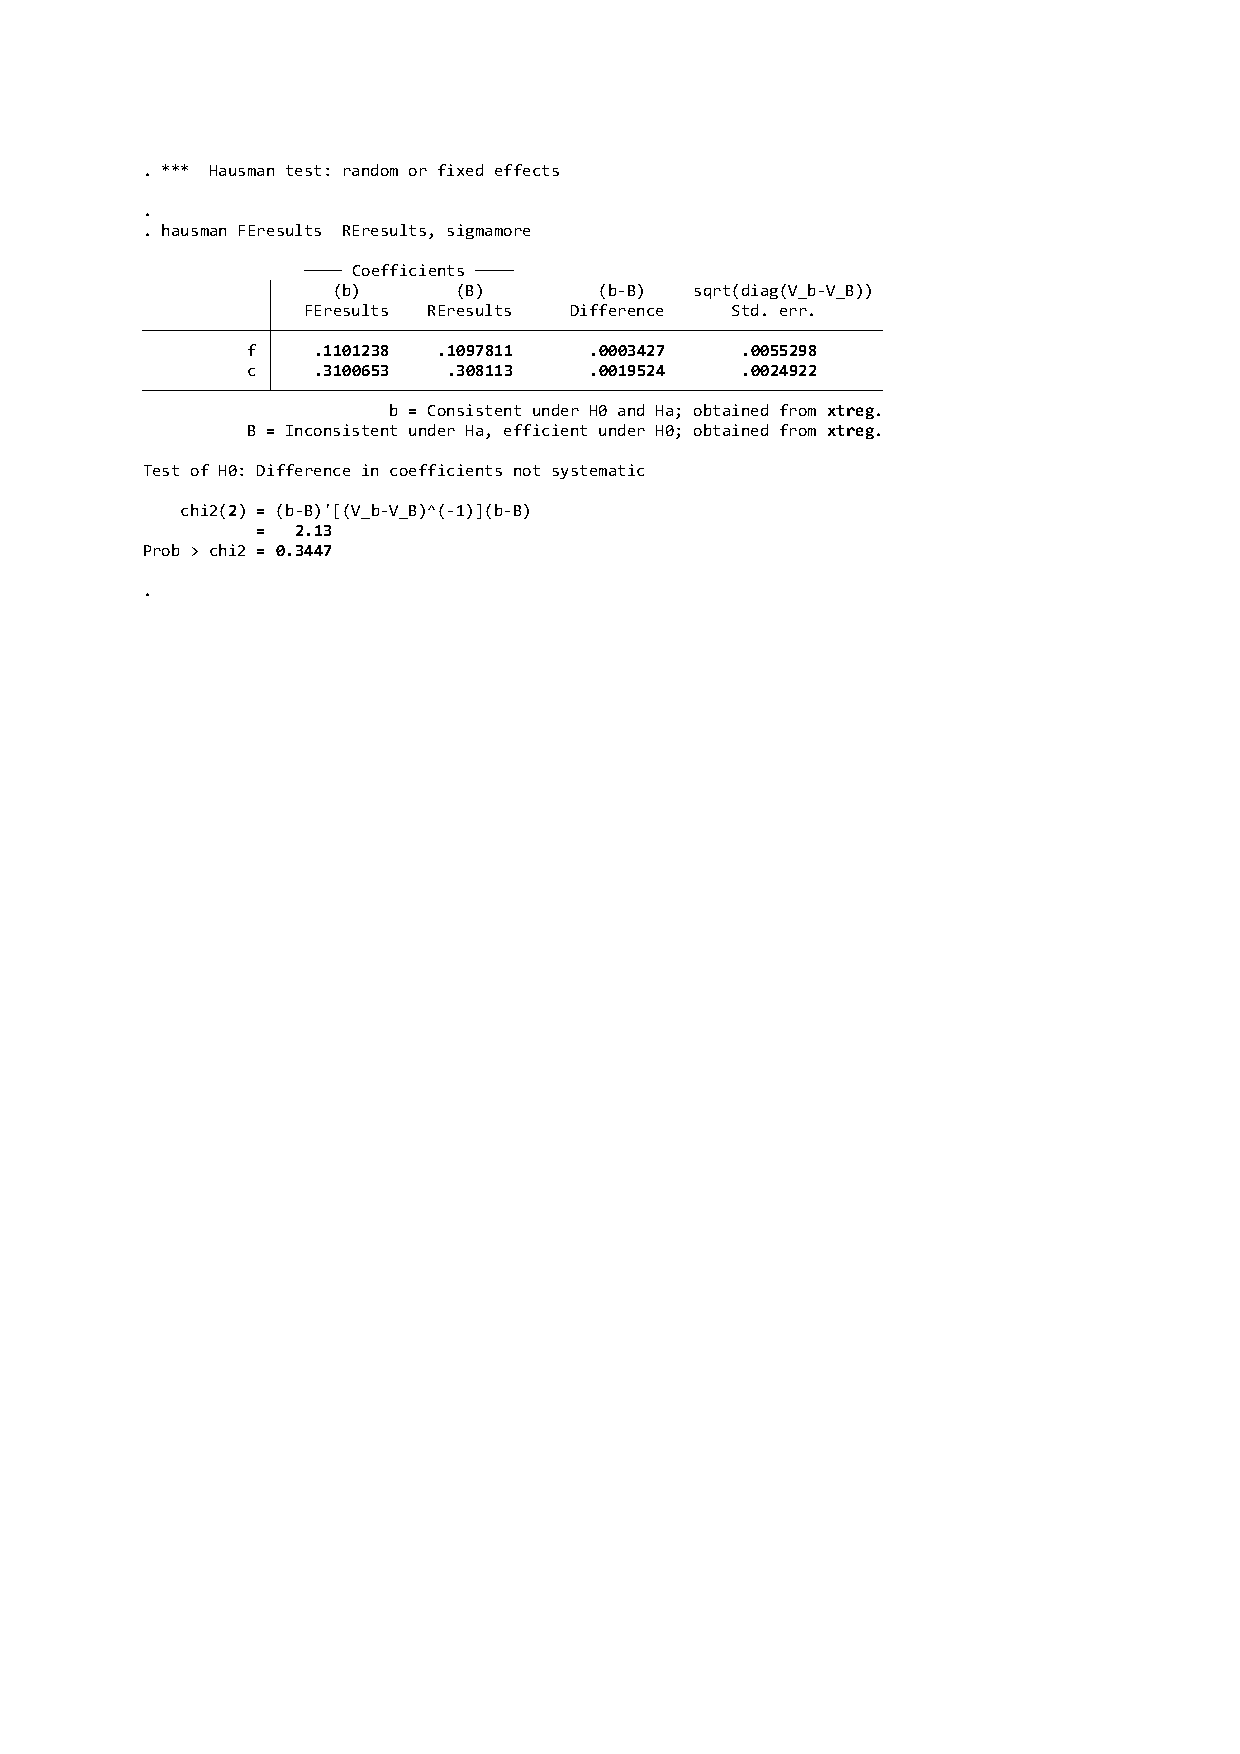
\includegraphics[width=\textwidth]{hh12.pdf}
\end{figure}
\end{frame}

\begin{frame}{Grunfeld - summary of results}
$$
\begin{array}{rccc}
&&\beta_1&\beta_2 \\
\text{Pooled OLS}&\Rightarrow& .1155622& .2306785\\
&&(.0058357)&(.0254758)\\\\
\text{Within FE estimator}&\Rightarrow& .1101238&.3100653\\
&&(.0118567)&(.0173545)\\\\
\text{RE estimator}&\Rightarrow&.1097811 &.308113\\
&&( .0104927)&(.0171805)\\
\end{array}
$$
\begin{itemize}
\item[$\Rightarrow$] Clearly pooled OLS sticks out, but the other two are quite similar (as expected based on the Hausman test)
\end{itemize}
\end{frame}


\end{document}

